\documentclass[border=10pt]{standalone}

\usepackage{tikz}
\usepackage{tikzsymbols}
\usetikzlibrary{calc,patterns,shapes.geometric}

\def\centerarc[#1](#2)(#3:#4:#5){\draw[#1] ($(#2)+({#5*cos(#3)},{#5*sin(#3)})$) arc (#3:#4:#5);}

\begin{document}
	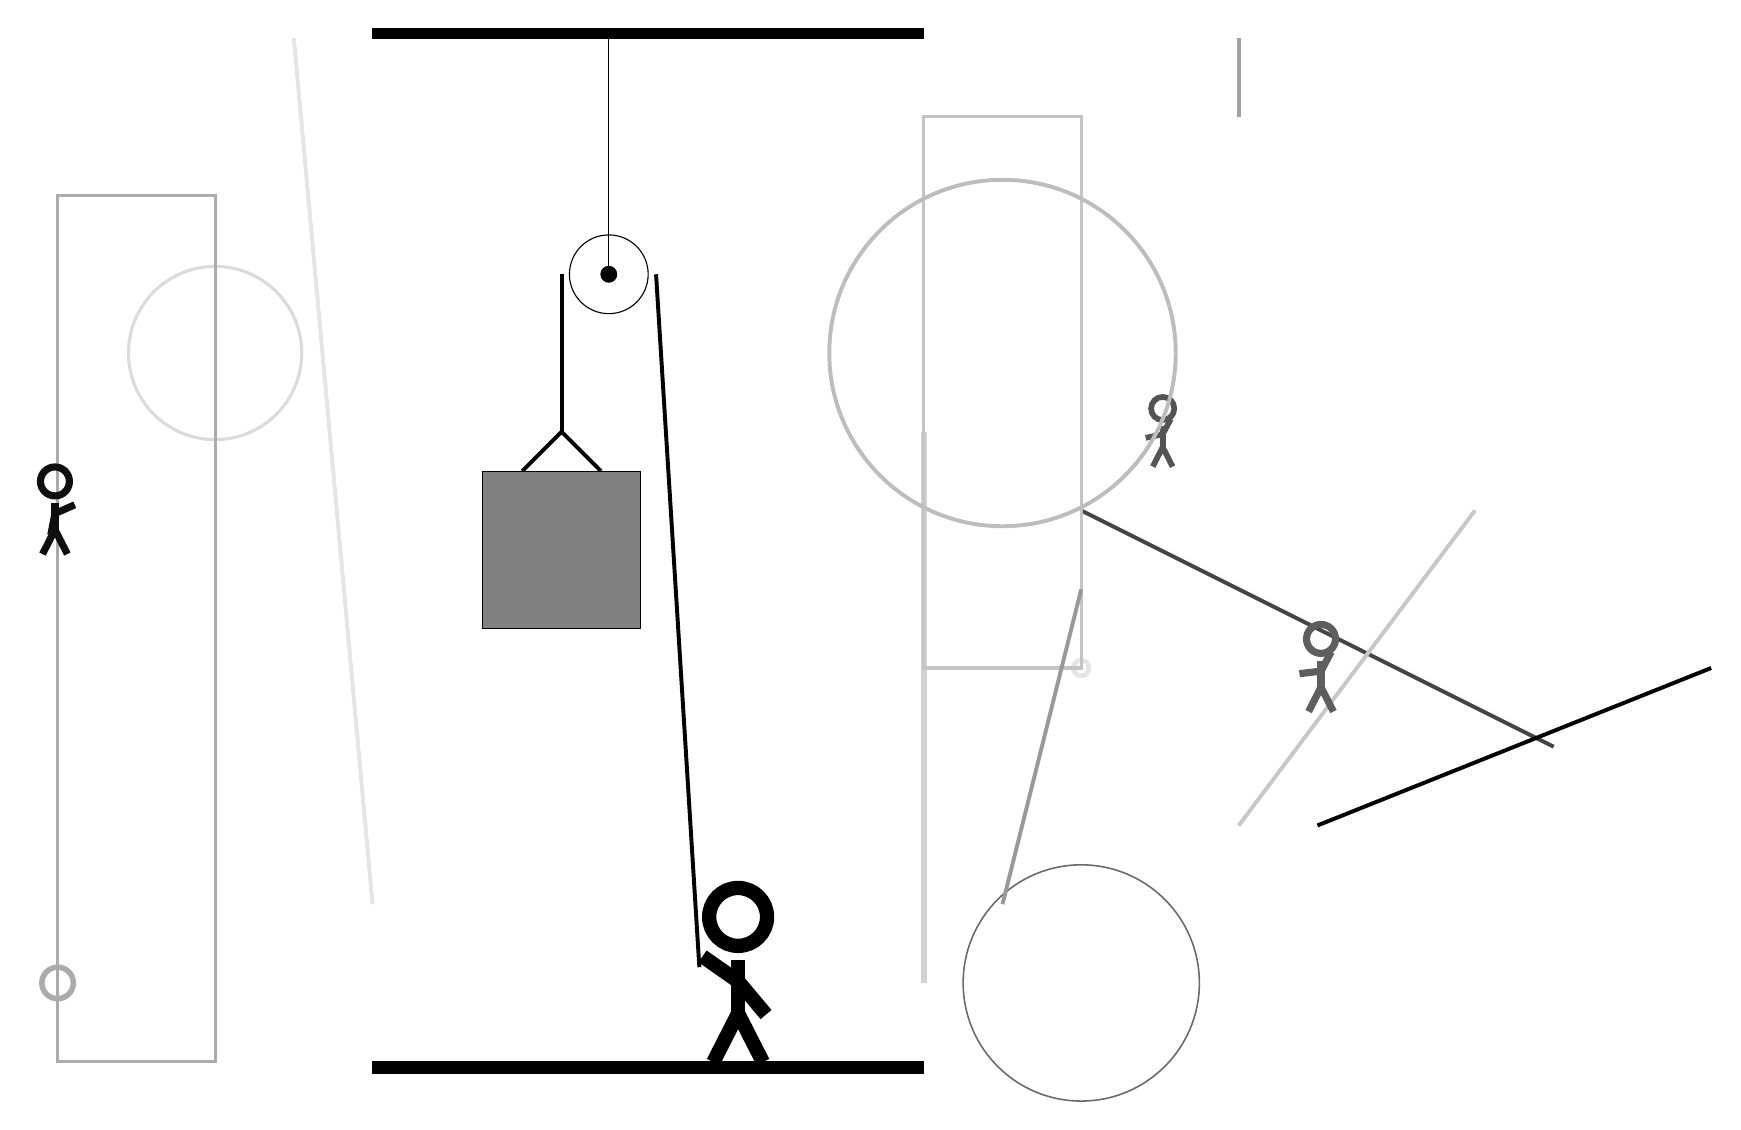
\begin{tikzpicture}
		%%%%% START %%%%%
		
		\draw[fill=black] (-2, 10) rectangle (5, 10.125);
		
		\draw[line width=0.7mm, color=black!18] (5, 5) rectangle (5, -2);
		
		\draw [line width=0.6mm, color=black!10](7, 2) circle (0.1);
		\draw[line width=0.2mm, color=black!80] (-4, 5) rectangle (-4, -3);
		\draw [line width=0.2mm, color=black!59](7, -2) circle (1.5);
		\draw [line width=0.4mm, color=black!14](-4, 6) circle (1.1);
		
		\draw[line width=0.5mm, color=black!10](-3, 10) -- (-2, -1);
		\draw[line width=0.5mm, color=black!73](7, 4) -- (13, 1);
		\draw[line width=0.4mm, color=black!23] (5, 9) rectangle (7, 2);
		\draw[line width=0.4mm, color=black!33] (-4, -3) rectangle (-6, 8);
		\draw [line width=0.7mm, color=black!33](-6, -2) circle (0.2);
		
		\node[line width=0.5mm, color=black!67] at (8, 5) {\Strichmaxerl[4][12][62]};
		\draw[line width=0.5mm, color=black!40](7, 3) -- (6, -1);
		\draw[line width=0.5mm, color=black!37](9, 10) -- (9, 9);
		\draw[line width=0.5mm, color=black!100](10, 0) -- (15, 2);
		\node[line width=0.3mm, color=black!94] at (-6, 4) {\Strichmaxerl[5][79][24]};
		\draw [line width=0.5mm, color=black!26](6, 6) circle (2.2);
		\draw[line width=0.5mm, color=black!22](9, 0) -- (12, 4);
		\node[line width=0.5mm, color=black!63] at (10, 2) {\Strichmaxerl[5][7][62]};
		
		\draw (1, 7) circle (0.5);
		\draw[fill=black] (1, 7) circle (0.1);
		\draw (1, 10) -- (1, 7);
		
		\draw[line width=0.5mm] (-0.1, 4.5) -- (0.4, 5.0) -- (0.9, 4.5);
		\draw[fill=black!50] (-0.6, 4.5) rectangle (1.4, 2.5);
		
		\draw[line width=0.5mm] (0.4, 7) -- (0.4, 5.0);
		\centerarc[line width=0.5mm](1, 7)(0:180:0.6);
		\draw[line width=0.5mm](1.6, 7) -- (2.15, -1.8);
		
		\node at (2.6, -1.9) {\Strichmaxerl[10][-35][-50]};
		
		\draw[fill=black] (-2, -3) rectangle (5, -3.15);
		
		%%%%% END %%%%%
	\end{tikzpicture}
\end{document}